\documentclass[../../main.tex]{subfiles}
 
\begin{document}

Radio-frequency (RF) phased array systems are examples of active electronically-scanned arrays (AESAs) that have applications in radar telemetry, telecommunications, ground-penetrating radar, scientific instrumentation, and remote sensing \cite{Vieregg_2016,AVVA201746,arnold_2020,PhysRevD.105.122006,10.3390/s21186091,10.1016/j.jappgeo.2022.104876,phased_array_book}.  All AESAs have \textit{radiation patterns} that define directions of maximum transmission power and received sensitivity, both due to constructive interferance of the transmitted or received RF plane wave.  Radiation patterns usually have a main lobe in which most of the radiation is concentrated, and the angular width of the main lobe is called the beam width.  In the one-dimensional case, $N$ three-dimensional RF antennas are arranged in a line with fixed spacing.  In the two-dimensional case, $N \times M$ three-dimensional antenna elements are arranged in a two-dimensional grid with fixed spacing in both dimensions.  The signal to noise ratio (SNR) of received signals in arrays of dimension $N$ is boosted by a factor of $\approx \sqrt{N}$, because the $N$ signals are combined coherently while thermal noise adds like $\sqrt{N}$.  The SNR boost is critical for certain kinds of scientific observations.  For example, systems created at the Center for Remote Sensing and Integrated Systems (CReSIS) are flown in polar regions to perform radar sounding of ice sheets for the purposes of geophysics and climate science \cite{arnold_2020}.  Radio signals transmitted from aircraft propagate downward through the ice.  Reflected signals carry information about the ice depth, temperature, and the presence of internal layers.  The radio echoes have small SNR values that require phased array receivers.  \\ \vspace{2.5mm}

Traditionally, phased array systems used in scientific projects are designed by hand, and commerical software is purchased to create the designs.  Proprietary computational electromagnetism (CEM) packages like XFDTD and HFSS are used to model the response of elements within phased arrays and the behavior of arrays \cite{remcom,ansys}.  The XFDTD package, for example, relies on the finite difference time domain (FDTD) method. The FDTD approach is a CEM technique in which spacetime and Maxwell’s equations are broken into discrete form.  HFSS uses a similar approach in the Fourier domain, called the Finite Element Method (FEM).  Depending on the software license and version, the current price of these CEM products ranges between \$5,000 and \$40,000 USD.  These costs are prohibitive for many academic institutions that primarily serve undergraduates, and Hispanic Serving Institutions like Whittier College.  Reducing this financial barrier to entry would enable diverse researchers to participate in the design process. \\ \vspace{2.5mm}

Aside from the cost, a drawback of commercial modeling software is the lack of access to the source code.  Having source code facilitates the incorporation of machine learning packages like NumPy and Scikit-Learn with the RF design process.  Phased array system properties can be optimized to a given application using machine learning.  These properties are determined by the 3D shape of the RF elements in the array, but the parameter space for RF element shapes is large.  Machine learning tools can be used to locate optimal solutions within this space as long as they can interface with the CEM software.  The authors of \cite{10.3390/electronics8121506} review a number of open-source CEM packages, and conclude that there are open-source options that match the performance of the commerical choices for simple RF antenna shapes.  Because Maxwell's equations are scale-invariant, open-source CEM packages designed for optical photonics can be used calculations at the cm-scale wavelengths relevant for particle astrophysics and geophysics.  One such open-source package is the MIT Electromagnetic Equation Propagation (MEEP) package \cite{10.1016/j.cpc.2009.11.008}.  We have shown that MEEP can drive the RF phased-array design process, and that 3D printer schematics can be extracted from this process \cite{electronics10040415,meepcon2022,10.1016/j.cpc.2009.11.008}. \\ \vspace{2.5mm}

Recent advances in materials research have led to the creation of 3D printer filament that has conductivities relevant for RF antenna production.  Resulting from an NSF Translational Impact (TI) award (1721644), Multi3D LLC. has produced filament with a resistivity of just 0.006 $\Omega$ cm: the Electrifi filament.  Several antenna designs have already been produced \cite{8786183,10.1049/iet-map.2017.0104}.  These examples include horn antennas with gain factors of 15 dB at 5.8 GHz, and microstrip patch antennas with gains of 1-2 dB at 2.5 GHz.  The results match expectations from HFSS models, exhibiting no major differences with antennas made using perfect conductors.  There are, however, virtually no examples of 3D printed RF phased arrays in the [0.1 - 1] GHz bandwidth.  This bandwidth is the most relevant for the aforementioned applications.  Further, the 3D printed results that take advantage of the Electrifi filament from Multi3D LLC appear to be well-known designs.  These designs can be optimized, and whole new designs can be discovered, by fully incorporating machine learning tools into the CEM packages used to model the RF elements.  In Sec. \ref{sec:cem}, we will review the progress already made at Whittier College along these lines.  In Sec. \ref{sec:askaryan}, we will show how this work will enhance the field of UHE-$\nu$ observations.  In Sec. \ref{sec:cresis}, we will show how this work will enhance the field of radio echo sounding of ice sheets and ice shelves.  In Sec. \ref{sec:onr}, we will show how this work can benefit active radar testing.  In Sec. \ref{sec:conc_im}, we make the case that the overall intellectual merits of the proposed activities are sound.

\section{Computational Electromagnetism and Additive Manufacturing}
\label{sec:cem}

In Summer 2020, we received a Summer Faculty Research Fellowship from the Office of Naval Research (ONR) to teach US Navy RF engineers about phased arrays in the [0.5 - 5] GHz bandwidth.  Whittier College is a member institution of the IceCube Gen2 collaboration, and we focus on the radio portion of the IceCube Gen2 design.  With our background in NSF-funded projects like ARIANNA, ARA, and NASA-funded projects like ANITA, we were qualified to teach our colleagues in the ONR about the applications of phased arrays.  Once the design process was understood, our goal was to design a phased array system that was to be integrated into an anechoic chamber.  The purpose of the anechoic chamber was to become a testing facility for active radar systems used in a Naval context.  We began by giving several one-hour lectures on the electromagnetism of phased arrays and applications within scientific research.  The audience included engineers and programmers working to acquire and develop RF systems for the Naval Surface Warfare Center (NSWC), Corona Division (NSWC Corona).  Our design flow is depicted in Fig. \ref{fig:design} below.  As the COVID-19 pandemic took hold, in-person work was stopped and funding for engineering development began to wane.  We made the decision to investigate open-source options for the CEM phase of the design. \\ \vspace{2.5mm}

\begin{figure}
\centering
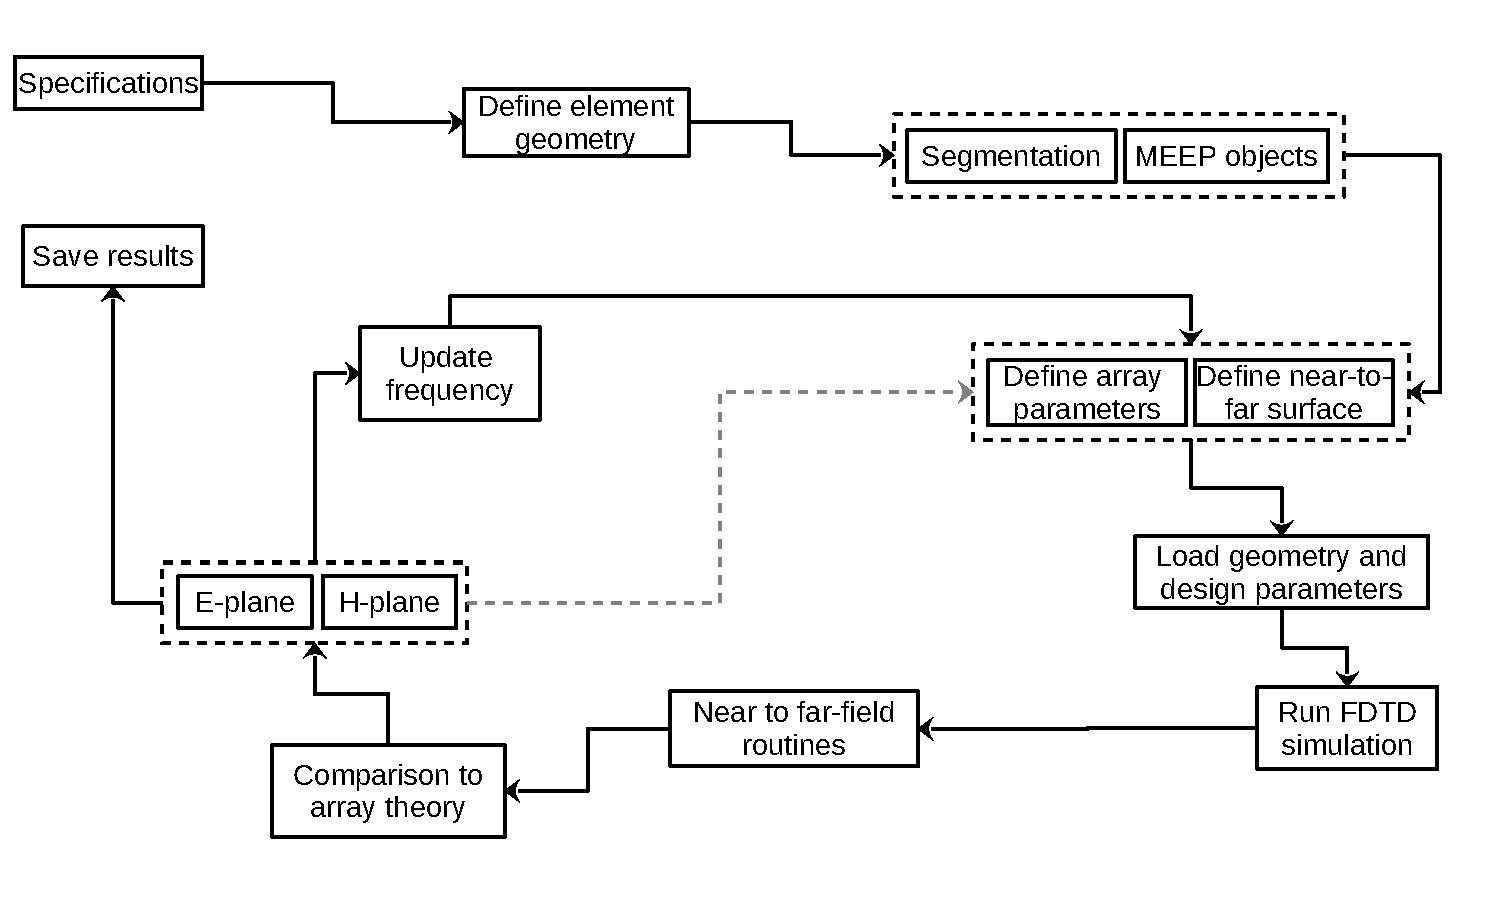
\includegraphics[width=0.85\textwidth]{diagram3.pdf}
\caption{\label{fig:design}  Our design process for RF phased arrays from \cite{electronics10040415}, adapted from Fig. 1 of the review \cite{10.3390/electronics8121506}.}
\end{figure}

We encountered a review article in the open-access journal \textit{Electronics} that indicated there are several open-source CEM tools that can be adapted for RF phased array analysis \cite{electronics10040415}.  Our design flow in Fig. \ref{fig:design} is adapted from Fig. 1 of the review to include specific tasks required for phased arrays, and near-to-far-field projections for the computation of radiation patterns.  MEEP was noted by the authors in the review as the most advanced among open-source FDTD programs.  The authors of the review did not benchmark it against HFSS or XFDTD due to the ``steep'' learning curve.  As part of the ONR Summer Faculty Fellowship, we decided to figure out how MEEP can be used to model RF systems.  The key insight was that MEEP takes advantage of the \textit{scale invariance} of Maxwell's Equations.  The simplest way to understand this is to understand how MEEP uses relative units when breaking Maxwell's equations into usable statements in algorithms and code. \\ \vspace{2.5mm}

Like other FDTD CEM methods, MEEP uses a Yee lattice to discretize Maxwell's equations \cite{10.1109/tap.1966.1138693}.  When the speed of light is set to unity ($c = 1$), distance and time units are set to be the same.  Frequency and wavelength units are the inverse of each other.  But distance and wavelength can take \textit{any} unit of length in the Yee lattice.  Most MEEP users interpret this unit of length to be 1 $\mu$m because the applications are for photonics.  For example, a \textit{relative} frequency (unit-less) of 0.5 corresponds to a \textit{relative} wavelength of 2.  When interpreted as 2 $\mu$m, the frequency is 150 THz in real units that correspond to optical bandwidth.  If we choose to interpret the \textit{relative} wavelength as 2 cm, the real frequency is 15 GHz.  A \textit{relative} frequency of 0.05 corresponds to the RF frequency 1.5 GHz.  Re-purposing MEEP from photonics simulator to RF simulator turned out to be simply a matter of interpretation. \\ \vspace{2.5mm}

\begin{figure}
\centering
%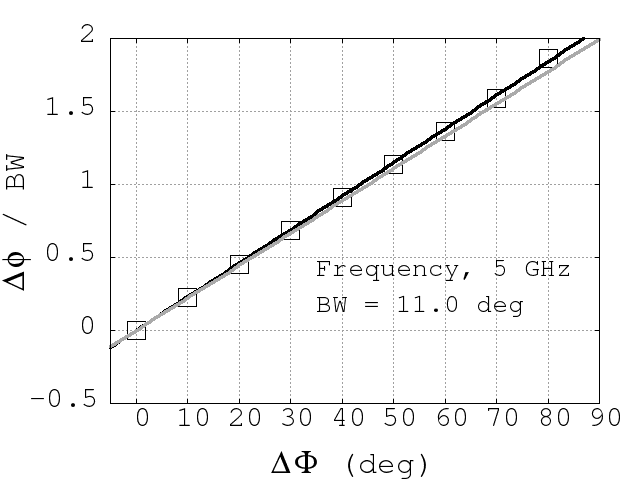
\includegraphics[width=0.35\textwidth]{figures/Oct30_plot2.png}
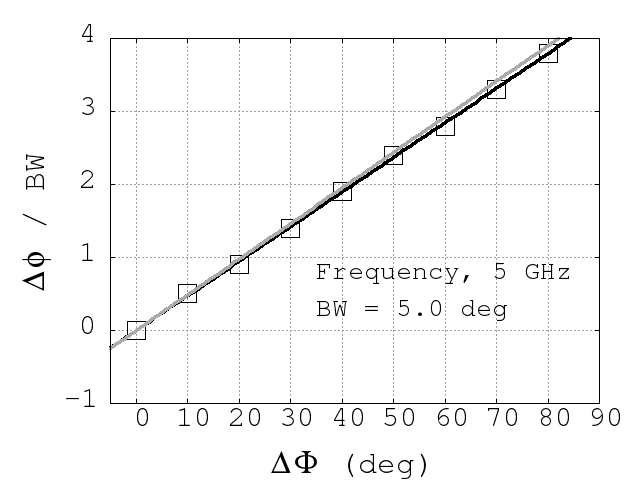
\includegraphics[width=0.33\textwidth]{figures/Oct30_plot1.png}
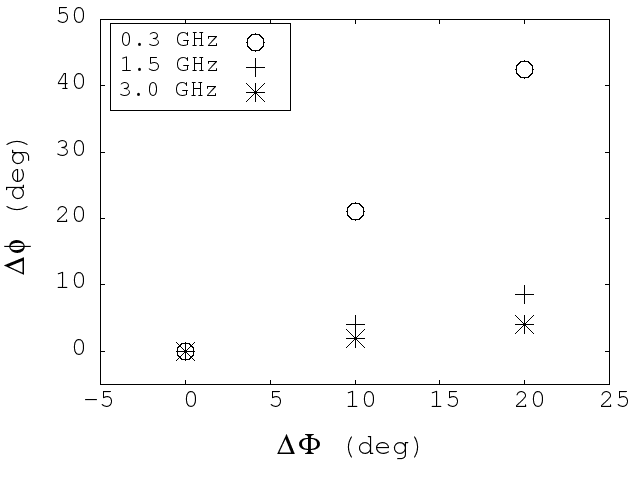
\includegraphics[width=0.33\textwidth]{figures/Aug11_plot2.png}
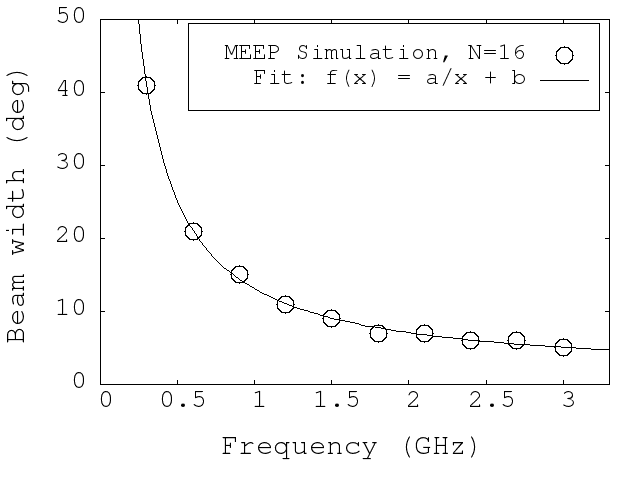
\includegraphics[width=0.33\textwidth]{figures/Aug11_plot1.png}
\caption{\label{fig:pa_1} (Left) The beam angle $\Delta \phi$ divided by the beam width $BW$ for the $N = 16$ one-dimensional Yagi array versus $\Delta \Phi$, the phase shift per element. (Middle) $\Delta \phi$ versus $\Delta \Phi$ for the $N=16$ version of the one-dimensional horn array, for several frequencies.  (Right) The dependence of the beam width on frequency for the one-dimensional $N=16$ horn array.}
\end{figure}

By Fall 2020, we were producing CEM models using MEEP that matched all expected properties of RF phased arrays.  For a one-dimensional array with $N$ RF elements, there is a linear relationship between the radiated plane-wave direction $\Delta \phi$, and the phase shift per RF element $\Delta \Phi$.  The coefficient of the relationship is determined by the ratio of real wavelength to RF element spacing.  Figure \ref{fig:pa_1} contains results for our first phased array models in which the single RF elements were Yagi-Uda style antennas and horn antennas.  The linear relationship is evident in the data.  The radiated signal direction $\Delta \phi$ is divided by the beam width (BW) in Fig. \ref{fig:pa_1} (left) and (middle) portions of the figure.  A beam width of a radiation pattern is the angular width of the main lobe of radiation, outside of which the radiated power has decreased by at least 3 dB.  In Fig. \ref{fig:pa_1} (left), the $N=16$ Yagi array can steer a 5 GHz plane wave up to four beam widths to the right or left of the forward direction.  Yagi-Uda style antennas are simple dipole arrays designed for a single frequency.  In Fig. \ref{fig:pa_1} (middle), results are shown for an $N=16$ array of horn antennas.  Since horn antennas are broadband radiators, the linear relationship is shown for 0.3, 1.5, and 3.0 GHz.  In Fig. \ref{fig:pa_1} (right), the expected inverse relationship between beam width and frequency for broadband phased arrays is shown. \\ \vspace{2.5mm}

We can also produce phased array radiation patterns with MEEP that match theoretical expectations.  The radiation pattern of a one-dimensional array of $N$ point sources of electromagnetic radiation can be derived using first principles \cite{electronics10040415}.  The \textit{pattern multiplication theorem} states that a one-dimensional phased array radiation pattern of $N$ identical RF elements will be that of a row of $N$ point sources, multiplied by the radiation pattern of the individual RF element.  In Fig. \ref{fig:1dhornresults2} (left and middle), the $N=16$ horn array is shown radiating in the E-plane (x-y plane) at an angle of 9 degrees with respect to the forward direction (x-axis).  The radiation pattern is shown in \ref{fig:1dhornresults2} (right).  The phase shift per horn and the ratio of wavelength to horn spacing combine to yield a beam direction of $\Delta \phi = 9$ degrees.  If no phase shift per horn is introduced, then $\Delta \phi = 0$ degrees and the plane wave radiates in the x-direction.  The blue curve in the polar plot represents the CEM radiation pattern from MEEP, while the red curve is the theoretical expectation from a row of $N$ point sources.  Though the row of point sources is symmetric, with a back lobe at $\Delta \phi = 180 - 9 = 171$ degrees, the pattern multiplication theorem dictates that the horn array should have no back lobe.  The individual horns suppress backward radiation (in the negative x-direction).  In the same publication, we also showed that two-dimensional arrays of Yagi-Uda and horn antennas matched theoretical expectations exactly.  Our revelation that the photonics code MEEP could be applied to one and two-dimensional RF phased array design in single-frequency and broadband applications led to the publication receiving Top 10 honors for December 2020 to May 2021 from the editors of \textit{Electronics Journal}.

\begin{figure}
\centering
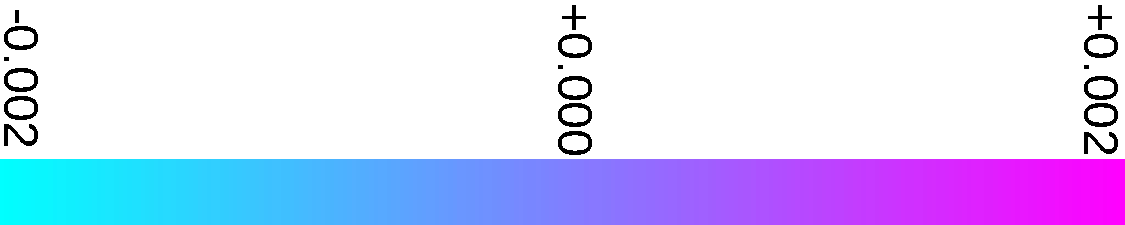
\includegraphics[width=5.625cm,angle=90]{figures/fields/colorbar.pdf}
%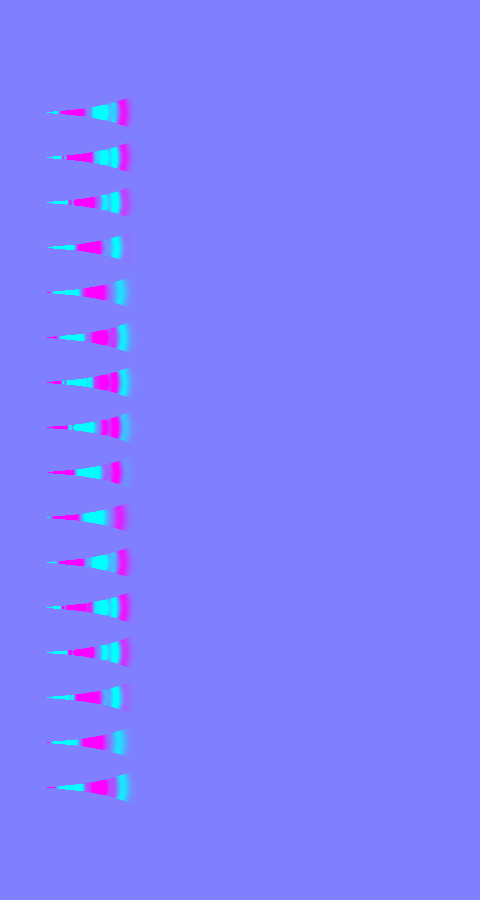
\includegraphics[width=3cm]{figures/fields/ey_phase_horn_t15.png}
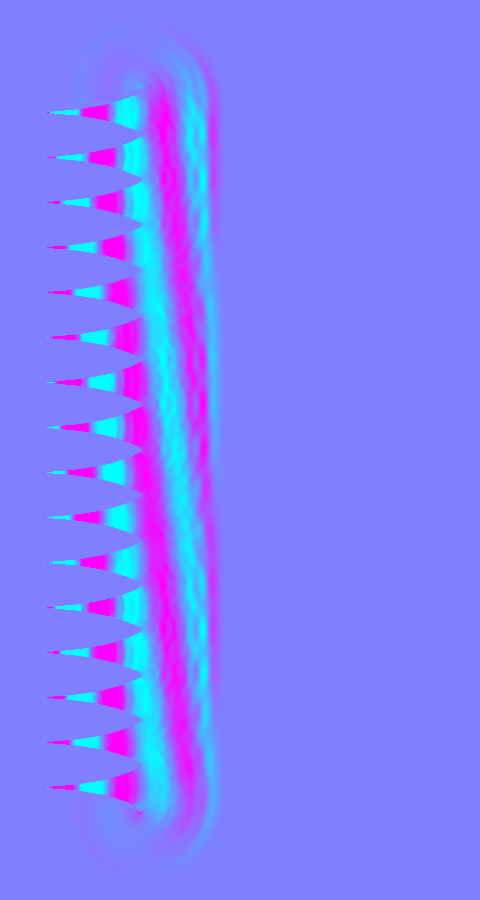
\includegraphics[width=3cm]{figures/fields/ey_phase_horn_t30.png}
%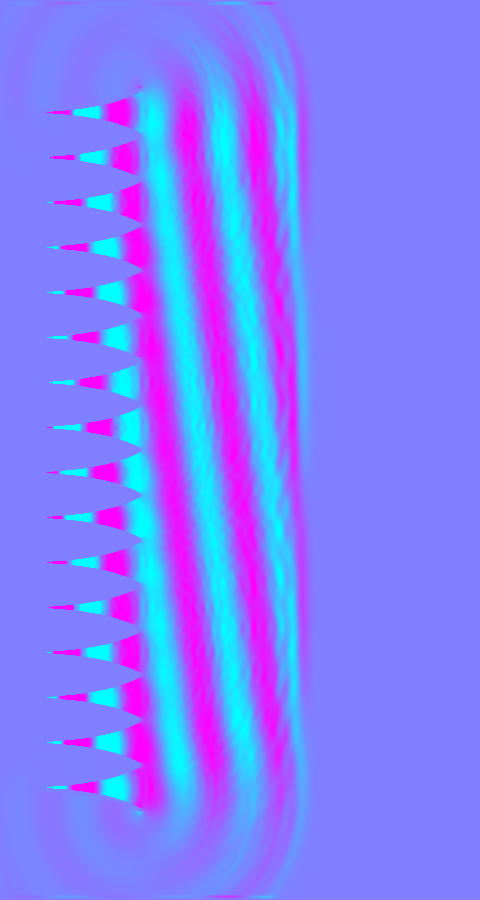
\includegraphics[width=3cm]{figures/fields/ey_phase_horn_t45.png}
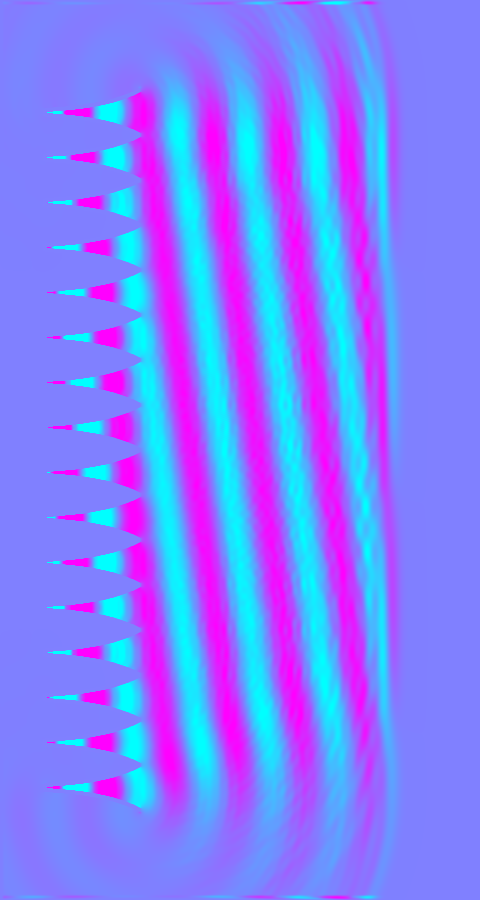
\includegraphics[width=3cm]{figures/fields/ey_phase_horn_t60.png}
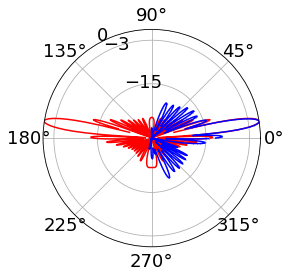
\includegraphics[width=6cm]{figures/fields/rad_patt_field.png}
\caption{\label{fig:1dhornresults2} (Left) The $N = 16$ one-dimensional horn array, radiating a linearly polarized electric field $|\vec{E}(x,y,t)|$ at $t = 1$ ns into the simulation run, and (middle) at $t = 2.0$ ns into the run.  The 2D area is $80 \times 150$ cm$^2$.  The frequency is 2.5 GHz, and the beam angle is $\Delta \phi = 9$ degrees from broadside (x-direction). (Right) The normalized radiated power versus $\Delta \phi$ known as the radiation pattern, in dB.  The blue curve represents the results from MEEP, and the red curve is the theoretical expectation from $N$ point sources.}
\end{figure}

In the same work, we showed that MEEP can be used to model the behavior of phased arrays in realistic polar ice environments.  Most commercial CEM packages assume a uniform ground plane and index of refraction in the medium surrounding the array.  By contrast, MEEP gives the user fine control of the index of refraction of each voxel, $n(x,y,z)$.  The RF index of refraction in polar ice is $n = 1.78$ for solid ice, but varies with the depth near the snow surface.  The transitional region between surface snow and solid ice in ice shelves and sheets in polar regions is known as the \textit{firn}.  The $n(z)$ function is well-measured in a variety of locations in Antarctica \cite{horizPaper}, and Greenland \cite{deaconu_2018}.  The ARA (South Pole) \cite{PhysRevD.105.122006}, Radio Neutrino Observatory, Greenland (RNO-G) \cite{rno}, and the proposed IceCube Gen2 project (South Pole) \cite{Aartsen_2021} all use or plan to use RF phased arrays as the primary UHE-$\nu$ detector.  The common simulation package used for these projects is NuRadioMC \cite{10.1140/epjc/s10052-020-7612-8}, which does not address the response of RF phased arrays in non-uniform media.  NuRadioMC addresses analytically the ray-tracing solution for UHE-$\nu$ signals as they propagate through polar ice.  We derived the analytic ray-tracing solutions presented in \cite{horizPaper} and \cite{10.1140/epjc/s10052-020-7612-8}, which were adopted into NuRadioMC.  The ray-tracing approach is an approximation that does not capture the precise behavior of three-dimensional field propagation in ice with realistic $n(x,y,z)$.  CEM tools that use the FDTD method offer a way to gain the necessary precision to match UHE-$\nu$ observations to computational predictions. ...

%things
%
%1. Impetus for the project and the ONR
%2. Review article
%3. Decision about MEEP
%4. The first paper, and accolades.  ICRC proceeding, and n(z)
%5. 3D printing with PLA and Multi3D LLC Electrifi
%	-Examples already created
%	-The design loop
%	-GDSII file formatting, kLayout and interfacing to 3D printing

\section{The Connection to Ultra-high Energy Neutrino Observations}
\label{sec:askaryan}

Example

\section{The Connection to Remote Sensing of Ice Sheets}
\label{sec:cresis}

Example

\section{The Connection to Office of Naval Research Projects}
\label{sec:onr}

Example

\section{Conclusion, Intellectual Merits}
\label{sec:conc_im}

Example

\end{document}
